% Options for packages loaded elsewhere
\PassOptionsToPackage{unicode}{hyperref}
\PassOptionsToPackage{hyphens}{url}
\PassOptionsToPackage{dvipsnames,svgnames,x11names}{xcolor}
%
\documentclass[
  letterpaper,
  DIV=11]{scrartcl}

\usepackage{amsmath,amssymb}
\usepackage{iftex}
\ifPDFTeX
  \usepackage[T1]{fontenc}
  \usepackage[utf8]{inputenc}
  \usepackage{textcomp} % provide euro and other symbols
\else % if luatex or xetex
  \usepackage{unicode-math}
  \defaultfontfeatures{Scale=MatchLowercase}
  \defaultfontfeatures[\rmfamily]{Ligatures=TeX,Scale=1}
\fi
\usepackage{lmodern}
\ifPDFTeX\else  
    % xetex/luatex font selection
\fi
% Use upquote if available, for straight quotes in verbatim environments
\IfFileExists{upquote.sty}{\usepackage{upquote}}{}
\IfFileExists{microtype.sty}{% use microtype if available
  \usepackage[]{microtype}
  \UseMicrotypeSet[protrusion]{basicmath} % disable protrusion for tt fonts
}{}
\makeatletter
\@ifundefined{KOMAClassName}{% if non-KOMA class
  \IfFileExists{parskip.sty}{%
    \usepackage{parskip}
  }{% else
    \setlength{\parindent}{0pt}
    \setlength{\parskip}{6pt plus 2pt minus 1pt}}
}{% if KOMA class
  \KOMAoptions{parskip=half}}
\makeatother
\usepackage{xcolor}
\setlength{\emergencystretch}{3em} % prevent overfull lines
\setcounter{secnumdepth}{-\maxdimen} % remove section numbering
% Make \paragraph and \subparagraph free-standing
\makeatletter
\ifx\paragraph\undefined\else
  \let\oldparagraph\paragraph
  \renewcommand{\paragraph}{
    \@ifstar
      \xxxParagraphStar
      \xxxParagraphNoStar
  }
  \newcommand{\xxxParagraphStar}[1]{\oldparagraph*{#1}\mbox{}}
  \newcommand{\xxxParagraphNoStar}[1]{\oldparagraph{#1}\mbox{}}
\fi
\ifx\subparagraph\undefined\else
  \let\oldsubparagraph\subparagraph
  \renewcommand{\subparagraph}{
    \@ifstar
      \xxxSubParagraphStar
      \xxxSubParagraphNoStar
  }
  \newcommand{\xxxSubParagraphStar}[1]{\oldsubparagraph*{#1}\mbox{}}
  \newcommand{\xxxSubParagraphNoStar}[1]{\oldsubparagraph{#1}\mbox{}}
\fi
\makeatother

\usepackage{color}
\usepackage{fancyvrb}
\newcommand{\VerbBar}{|}
\newcommand{\VERB}{\Verb[commandchars=\\\{\}]}
\DefineVerbatimEnvironment{Highlighting}{Verbatim}{commandchars=\\\{\}}
% Add ',fontsize=\small' for more characters per line
\usepackage{framed}
\definecolor{shadecolor}{RGB}{241,243,245}
\newenvironment{Shaded}{\begin{snugshade}}{\end{snugshade}}
\newcommand{\AlertTok}[1]{\textcolor[rgb]{0.68,0.00,0.00}{#1}}
\newcommand{\AnnotationTok}[1]{\textcolor[rgb]{0.37,0.37,0.37}{#1}}
\newcommand{\AttributeTok}[1]{\textcolor[rgb]{0.40,0.45,0.13}{#1}}
\newcommand{\BaseNTok}[1]{\textcolor[rgb]{0.68,0.00,0.00}{#1}}
\newcommand{\BuiltInTok}[1]{\textcolor[rgb]{0.00,0.23,0.31}{#1}}
\newcommand{\CharTok}[1]{\textcolor[rgb]{0.13,0.47,0.30}{#1}}
\newcommand{\CommentTok}[1]{\textcolor[rgb]{0.37,0.37,0.37}{#1}}
\newcommand{\CommentVarTok}[1]{\textcolor[rgb]{0.37,0.37,0.37}{\textit{#1}}}
\newcommand{\ConstantTok}[1]{\textcolor[rgb]{0.56,0.35,0.01}{#1}}
\newcommand{\ControlFlowTok}[1]{\textcolor[rgb]{0.00,0.23,0.31}{\textbf{#1}}}
\newcommand{\DataTypeTok}[1]{\textcolor[rgb]{0.68,0.00,0.00}{#1}}
\newcommand{\DecValTok}[1]{\textcolor[rgb]{0.68,0.00,0.00}{#1}}
\newcommand{\DocumentationTok}[1]{\textcolor[rgb]{0.37,0.37,0.37}{\textit{#1}}}
\newcommand{\ErrorTok}[1]{\textcolor[rgb]{0.68,0.00,0.00}{#1}}
\newcommand{\ExtensionTok}[1]{\textcolor[rgb]{0.00,0.23,0.31}{#1}}
\newcommand{\FloatTok}[1]{\textcolor[rgb]{0.68,0.00,0.00}{#1}}
\newcommand{\FunctionTok}[1]{\textcolor[rgb]{0.28,0.35,0.67}{#1}}
\newcommand{\ImportTok}[1]{\textcolor[rgb]{0.00,0.46,0.62}{#1}}
\newcommand{\InformationTok}[1]{\textcolor[rgb]{0.37,0.37,0.37}{#1}}
\newcommand{\KeywordTok}[1]{\textcolor[rgb]{0.00,0.23,0.31}{\textbf{#1}}}
\newcommand{\NormalTok}[1]{\textcolor[rgb]{0.00,0.23,0.31}{#1}}
\newcommand{\OperatorTok}[1]{\textcolor[rgb]{0.37,0.37,0.37}{#1}}
\newcommand{\OtherTok}[1]{\textcolor[rgb]{0.00,0.23,0.31}{#1}}
\newcommand{\PreprocessorTok}[1]{\textcolor[rgb]{0.68,0.00,0.00}{#1}}
\newcommand{\RegionMarkerTok}[1]{\textcolor[rgb]{0.00,0.23,0.31}{#1}}
\newcommand{\SpecialCharTok}[1]{\textcolor[rgb]{0.37,0.37,0.37}{#1}}
\newcommand{\SpecialStringTok}[1]{\textcolor[rgb]{0.13,0.47,0.30}{#1}}
\newcommand{\StringTok}[1]{\textcolor[rgb]{0.13,0.47,0.30}{#1}}
\newcommand{\VariableTok}[1]{\textcolor[rgb]{0.07,0.07,0.07}{#1}}
\newcommand{\VerbatimStringTok}[1]{\textcolor[rgb]{0.13,0.47,0.30}{#1}}
\newcommand{\WarningTok}[1]{\textcolor[rgb]{0.37,0.37,0.37}{\textit{#1}}}

\providecommand{\tightlist}{%
  \setlength{\itemsep}{0pt}\setlength{\parskip}{0pt}}\usepackage{longtable,booktabs,array}
\usepackage{calc} % for calculating minipage widths
% Correct order of tables after \paragraph or \subparagraph
\usepackage{etoolbox}
\makeatletter
\patchcmd\longtable{\par}{\if@noskipsec\mbox{}\fi\par}{}{}
\makeatother
% Allow footnotes in longtable head/foot
\IfFileExists{footnotehyper.sty}{\usepackage{footnotehyper}}{\usepackage{footnote}}
\makesavenoteenv{longtable}
\usepackage{graphicx}
\makeatletter
\newsavebox\pandoc@box
\newcommand*\pandocbounded[1]{% scales image to fit in text height/width
  \sbox\pandoc@box{#1}%
  \Gscale@div\@tempa{\textheight}{\dimexpr\ht\pandoc@box+\dp\pandoc@box\relax}%
  \Gscale@div\@tempb{\linewidth}{\wd\pandoc@box}%
  \ifdim\@tempb\p@<\@tempa\p@\let\@tempa\@tempb\fi% select the smaller of both
  \ifdim\@tempa\p@<\p@\scalebox{\@tempa}{\usebox\pandoc@box}%
  \else\usebox{\pandoc@box}%
  \fi%
}
% Set default figure placement to htbp
\def\fps@figure{htbp}
\makeatother
% definitions for citeproc citations
\NewDocumentCommand\citeproctext{}{}
\NewDocumentCommand\citeproc{mm}{%
  \begingroup\def\citeproctext{#2}\cite{#1}\endgroup}
\makeatletter
 % allow citations to break across lines
 \let\@cite@ofmt\@firstofone
 % avoid brackets around text for \cite:
 \def\@biblabel#1{}
 \def\@cite#1#2{{#1\if@tempswa , #2\fi}}
\makeatother
\newlength{\cslhangindent}
\setlength{\cslhangindent}{1.5em}
\newlength{\csllabelwidth}
\setlength{\csllabelwidth}{3em}
\newenvironment{CSLReferences}[2] % #1 hanging-indent, #2 entry-spacing
 {\begin{list}{}{%
  \setlength{\itemindent}{0pt}
  \setlength{\leftmargin}{0pt}
  \setlength{\parsep}{0pt}
  % turn on hanging indent if param 1 is 1
  \ifodd #1
   \setlength{\leftmargin}{\cslhangindent}
   \setlength{\itemindent}{-1\cslhangindent}
  \fi
  % set entry spacing
  \setlength{\itemsep}{#2\baselineskip}}}
 {\end{list}}
\usepackage{calc}
\newcommand{\CSLBlock}[1]{\hfill\break\parbox[t]{\linewidth}{\strut\ignorespaces#1\strut}}
\newcommand{\CSLLeftMargin}[1]{\parbox[t]{\csllabelwidth}{\strut#1\strut}}
\newcommand{\CSLRightInline}[1]{\parbox[t]{\linewidth - \csllabelwidth}{\strut#1\strut}}
\newcommand{\CSLIndent}[1]{\hspace{\cslhangindent}#1}

\usepackage{float}
\usepackage{tabularray}
\usepackage[normalem]{ulem}
\usepackage{graphicx}
\UseTblrLibrary{booktabs}
\UseTblrLibrary{rotating}
\UseTblrLibrary{siunitx}
\NewTableCommand{\tinytableDefineColor}[3]{\definecolor{#1}{#2}{#3}}
\newcommand{\tinytableTabularrayUnderline}[1]{\underline{#1}}
\newcommand{\tinytableTabularrayStrikeout}[1]{\sout{#1}}
\KOMAoption{captions}{tableheading}
\makeatletter
\@ifpackageloaded{caption}{}{\usepackage{caption}}
\AtBeginDocument{%
\ifdefined\contentsname
  \renewcommand*\contentsname{Inhaltsverzeichnis}
\else
  \newcommand\contentsname{Inhaltsverzeichnis}
\fi
\ifdefined\listfigurename
  \renewcommand*\listfigurename{Abbildungsverzeichnis}
\else
  \newcommand\listfigurename{Abbildungsverzeichnis}
\fi
\ifdefined\listtablename
  \renewcommand*\listtablename{Tabellenverzeichnis}
\else
  \newcommand\listtablename{Tabellenverzeichnis}
\fi
\ifdefined\figurename
  \renewcommand*\figurename{Abbildung}
\else
  \newcommand\figurename{Abbildung}
\fi
\ifdefined\tablename
  \renewcommand*\tablename{Tabelle}
\else
  \newcommand\tablename{Tabelle}
\fi
}
\@ifpackageloaded{float}{}{\usepackage{float}}
\floatstyle{ruled}
\@ifundefined{c@chapter}{\newfloat{codelisting}{h}{lop}}{\newfloat{codelisting}{h}{lop}[chapter]}
\floatname{codelisting}{Listing}
\newcommand*\listoflistings{\listof{codelisting}{Listingverzeichnis}}
\makeatother
\makeatletter
\makeatother
\makeatletter
\@ifpackageloaded{caption}{}{\usepackage{caption}}
\@ifpackageloaded{subcaption}{}{\usepackage{subcaption}}
\makeatother

\ifLuaTeX
\usepackage[bidi=basic]{babel}
\else
\usepackage[bidi=default]{babel}
\fi
\babelprovide[main,import]{ngerman}
% get rid of language-specific shorthands (see #6817):
\let\LanguageShortHands\languageshorthands
\def\languageshorthands#1{}
\ifLuaTeX
  \usepackage[german]{selnolig} % disable illegal ligatures
\fi
\usepackage{bookmark}

\IfFileExists{xurl.sty}{\usepackage{xurl}}{} % add URL line breaks if available
\urlstyle{same} % disable monospaced font for URLs
\hypersetup{
  pdftitle={Was kennzeichnet Professionalität in der Deutsch-Fachdidaktik (Sprache)?},
  pdflang={de},
  pdfkeywords={Professionalität, Fachdidaktik, Lehrpersonenbildung, Natural
Language Processing},
  colorlinks=true,
  linkcolor={blue},
  filecolor={Maroon},
  citecolor={Blue},
  urlcolor={Blue},
  pdfcreator={LaTeX via pandoc}}


\title{Was kennzeichnet Professionalität in der Deutsch-Fachdidaktik
(Sprache)?}
\usepackage{etoolbox}
\makeatletter
\providecommand{\subtitle}[1]{% add subtitle to \maketitle
  \apptocmd{\@title}{\par {\large #1 \par}}{}{}
}
\makeatother
\subtitle{Analysen offen und geschlossen erfasster Überzeugungen von
Deutschlehrkräften.}
\author{Samuel Merk \and Colin Cramer}
\date{2025-01-06}

\begin{document}
\maketitle
\begin{abstract}
``Professionalität'' von Lehrkräften wird einerseits
bildungswissenschaftlich theoretisiert und modelliert (z.B. im sog.
kompetenzorientierten oder im strukturtheoretischen Ansatz),
andererseits haben Lehrkräfte Überzeugungen bzgl. der Frage, was
Professionalität in ihrem Beruf ausmacht. Der vorliegende Beitrag
untersucht, inwiefern diese Überzeugungen den bildungswissenschaftlichen
Ansätzen ähnlich sind und ob sie spezifisch für einen fachdidaktischen
Kontext sind. In einem faktorenanalytischen Ansatz zeigten sich
Überzeugungen zu Professionalität in der Fachdidaktik Deutsch als
metrisch invariant gegenüber allgemeiner Professionalitätsüberzeugungen,
wichen jedoch substantiell von der a priori Struktur der
bildungswissenschaftlichen Ansätze ab. Word Embeddings von
Freitextantworten zeigten jedoch gleichzeitig eine Korrespondenz zu der
bildungswissenschaftlich implizierten Gliederung. Inwiefern aus diesen
Befunden auf eine kognitive Repräsentation bildungswissenschaftlicher
Professionalitätsansätze in den Überzeugungen von Lehrkräften
geschlossen werden kann, wird diskutiert.
\end{abstract}


\subsection{Einleitung (3k)}\label{einleitung-3k}

Die bildungswissenschaftliche Forschung hat sich intensiv mit der Frage
nach der Professionalität von Lehrkräften auseinandergesetzt und dabei
diverse, oft komplementäre Theorien und Konzepte generiert (Colin
Cramer, Ophoff, und Schreiber 2023). Während z.B. soziologisch
inspirierte Arbeiten für die Profession charakteristische Antinomien
identifizierten , topologisierten Arbeiten aus der pädagogischen
Psychologie Wissensbestände, Überzeugungen und motivationale Variablen
die sich in der Literatur als prädiktiv für Outcomes auf Ebene der
Schülerinnen und Schüler zeigten (Baumert und Kunter 2006; Krauss u.~a.
2004; Shulman 1986). Weitere Forschungsstränge bearbeiteten etwa in der
Tradition erziehungswissenschaftlicher Biografieforschung (Bauer 2000;
E. Terhart 1992) die besondere Bedeutung von berufsbiografischen
Übergängen und fassten Professionalität unter anderem als Sensibilität
für die Bedeutung der eigenen Biografie und das kontinuierliche
Bewältigen aktueller berufsbiografischer Herausforderungen auf. Die
Frage nach Professionalität im Lehrerinnen- und Lehrerberuf hat auch
Eingang in die Bildungsstandards der Ständigen Konferenz der
Kultusminister der Länder in der Bundesrepublik Deutschland gefunden.
Dementsprechend werden an Universitäten und pädagogischen Hochschulen
die zuvor genannten bildungswissenschaftlichen Professionalitätsansätze
gelehrt (Hohenstein u.~a. 2014). Es kann jedoch begründet angenommen
werden, dass Lehrkräfte in diesen Lernsituationen umfangreiche, bereits
bestehende implizite wie explizite Überzeugungen (Fives und Buehl 2012;
Merk 2020) bzgl. der Frage der Professionalität einbringen. Dies hätte
Konsequenzen für die Professionalisierungspraxis (Colin Cramer, Ophoff,
und Schreiber 2023), da diese Überzeugungen etwa über die ihnen
zugeschriebene Filter-, Rahmungs- und Handlungsleitungsfunktion (Fives
und Buehl 2012) dazu führen können, dass (angehende) Lehrkräfte
bestimmte Lerngelegenheiten unterschiedlich wählen und nutzen.
Dementsprechend liegt erste Forschung vor, die untersucht, inwiefern
Überzeugungen zur Professionalität von Lehrkräften in ihrer Struktur den
bildungswissenschaftlichen Theorien entspricht, wobei die Ergebnisse
sowohl auf Ähnlichkeiten und Abweichungen zwischen Überzeugungsstruktur
und Theorien hinweisen (Colin Cramer, Ophoff, und Schreiber 2023). Die
Ambiguität dieser Ergebnisse, deren unklare Generalisierbarkeit sowie
die grundsätzliche Diskussion um die Erfassbarkeit von Überzeugungen zu
Professionalität mit geschlossenen Fragebogenitems (Merk und Schmidt
2023) nimmt die vorliegende Studie zum Anlass um a) zu versuchen, die
von Cramer et al. (2023) gefundene Faktorenstruktur der
Professionalitätsüberzeugungen domänenspezifisch zu replizieren b) die
Faktorenstruktur von allgemeinen Professionalitätsüberzeugungen und
Professioalitätsüberzeugungen in der Fachdidaktik zu vergleichen und b)
die Ähnlichkeit des Inhalts von offen erfassten Überzeugungen und
bildungswissenschaftlichen Theorien zur Professionalität von Lehrerinnen
und Lehrern mit Natural Language Processing Methoden (Bittermann und
Fischer 2024) zu untersuchen.

\subsection{Theoretischer Hintergrund
(8K)}\label{theoretischer-hintergrund-8k}

\subsubsection{Professionalität von
Lehrkräften}\label{sec-professionalitat-von-lehrkraften}

In den Bildungswissenschaften ist in den letzten zwei Dekaden eine
lebendige, teils auch kontroverse Diskussion um die Charakteristika
professionellen Handelns im Lehrerberuf zu verzeichnen, die verschiedene
Ansätze zur Beschreibung von Professionalität hervorgebracht hat, welche
im Folgenden beschrieben werden sollen.

\paragraph{Strukturtheoretischer
Ansatz}\label{strukturtheoretischer-ansatz}

Ausgehend von soziologisch geprägten Arbeiten Oevermanns (1996) wirft
der strukturtheoretische Ansatz der Professionalität von Lehrkräften ein
besonderes Augenmerk auf die beruflichen Rahmenbedingungen von
Lehrerinnen und Lehrern wie etwa Rollenerwartungen oder soziale Gefüge
(Helsper 2014). In der Rezeption dieses Ansatzes haben sogenannte
``Antinomien'' oder ``professionelle Paradoxien'' des Lehrerinnen- und
Lehrerberufes besondere Aufmerksamkeit erfahren (Baumert und Kunter
2006). Sie beschreiben nicht auflösbare, aber charakteristische
Widersprüche in den professionellen Anforderungen wie etwa die simultane
Erfordernis von Nähe und Distanz zwischen Lehrkräften und Schülerinnen
und Schülern.

\paragraph{Kompetenzorientierter
Ansatz}\label{kompetenzorientierter-ansatz}

Der kompetenzorientierte Ansatz hingegen versucht, Wissensbestände,
Überzeugungen, motivationale Orientierungen und selbstregulative
Fähigkeiten von Lehrkräften zu systematisieren, die ein erfolgreicheres
Handeln wahrscheinlicher machen. Dabei wird Erfolg meist als gesteigerte
(operationaliserbare) Outcomes auf Ebene der Schülerinnen und Schüler
definiert, wie z.B. deren akademische Leistung oder Motivation. Diese
Systematisierung steht in der Tradition der Wissenstopologie Shulmans
(1986) und des Expertiseansatzes der Lehrerprofessionalität (Bromme
1992). Häufig zitiert werden Topologien, welche die für professionelle
Kompetenz konstitutiven Wissensdomänen Fachwissen, Fachdidaktisches
Wissen, Pädagogisches Wissen, Organisationales Wissen und
Beratungswissen jeweils in disjunkte Subdomänen unterteilen (Baumert und
Kunter 2006; König 2020; Krauss u.~a. 2004)

\paragraph{Berufsbiografischer Ansatz}\label{berufsbiografischer-ansatz}

In der Tradition erziehungswissenschaftlicher Biografieforschung
fokussieren Arbeiten die dem berufsbiografischen Ansatz zugeordnet
werden (z.B. Bauer, 2000a; Terhart, 2001) (Bauer 2000; Ewald Terhart
2001) eine stark intraindividuelle Perspektive: Sie betonen, dass
Professionalität von Lehrerinnen und Lehrern als ``berufsbiographisches
Entwicklungsproblem'' zu sehen sei (Ewald Terhart 1995, pp.~238) und
leiten daraus die Notwendigkeit einer Sensibilität für die eigene
Berufsbiografie, einer besonderen Berücksichtigung beruflicher Übergänge
(etwa zu Beginn des Referendariats) oder des Aufbaus eines beruflichen
Selbsts ab.

\paragraph{Metareflexiver Ansatz}\label{metareflexiver-ansatz}

Die bisher genannten Ansätze haben (neben weiteren) längst Eingang in
die institutionalisierte Lehrkräftebildung gefunden. Dies nahmen Cramer
et al. (2019) zum Anlass, Professionalität als mehrperspektivische
Betrachtung des eigenen Handelns unter Berücksichtigung aller drei
bisher genannter Ansätze sowie deren Unterschiede und Gemeinsamkeiten zu
definieren. Danach rekurrieren professionelle Lehrkräfte beim Treffen
von Entscheidungen auf Handlungsoptionen, die im Lichte \ldots. adäquat
erscheinen. Dabei reflektieren sie verschiedene Handlungsoptionen nicht
nur mehrperspektivisch entlang verschiedener situationsadäquater
Theorien und Konzepte, sondern auch deren terminologische Differenzen
und differentielle Axiomatiken (Colin Cramer, Brown, und Aldridge 2023).

\subsection{Überzeugungen von
Lehrkräften}\label{uxfcberzeugungen-von-lehrkruxe4ften}

Überzeugungen von Lehrkräften sind ein beliebter Forschungsgegenstand
(Fives u.~a. 2019; Pajares 1992; Skott 2015) in der Lehrerinnen- und
Lehrerbildungsforschung. Überzeugungen werden zum einen als sehr
wirkmächtig konzeptualisert - ihnen wird etwa eine Filter- Rahmungs- und
Handlungsleitungsfunktion zugeschrieben (Fives u.~a. 2019). Andererseits
gelten sie als vergleichsweise ökonomisch via Fragebogen erfassbar (Merk
2020). Da Überzeugungen meist als subjektive Wahrheitspropositionen
definiert werden (Skott 2015), liegt es nahe, die Forschung zu
Überzeugungen von Lehrerinnen und Lehrern nach dem Gegenstandsbereich
der Wahrheitspropositionen zu gliedern: Also etwa lehr- lerntheoretische
Überzeugungen (Dubberke u.~a. 2008; Turner, Christensen, und Meyer 2009;
Reusser und Pauli 2014), epistemische Überzeugungen (Blömeke u.~a. 2008;
Fives und Buehl 2008; Hofer und Bendixen 2012), Überzeugungen zu
heterogenen Lerngruppen (Gebauer, McElvany, und Klukas 2013) oder eben
Überzeugungen zur Professionalität von Lehrkräften (Colin Cramer,
Ophoff, und Schreiber 2023). Überzeugungen zu verschiedenen
Gegenstandsbereichen gelten jedoch als teilweise abhängig voneinander,
wenngleich nicht notwendigerweise konsistent: So weisen Lehrkräfte die
hochgradig transmissive Lerntheoretische Überzeugungen für das Fach
Mathematik aufweisen auch eher transmissive Lerntheoretische
Überzeugungen für das Fach Physik auf (Abhängigkeit), gleichzeitig gibt
es Evidenz dafür, dass Lehrkräfte davon überzeugt sind, dass es wichtig
ist ihre Praxis durch bildungswissenschaftliche Forschungsergebnisse zu
informieren, ohne dies jedoch auch umzusetzen (Gold, Thomm, und Bauer
2024; Walker, Nelson, und Bradshaw 2019). Für diese Domänenspezifität
und Kontextabhängigkeit von Überzeugungen liegen (insbesondere für
epistemische Überzeugungen) umfassende Rahmenmodelle vor (Merk u.~a.
2017; Muis, Bendixen, und Haerle 2006).

\subsubsection{Professionalitätsüberzeugungen von
Lehrkräften}\label{professionalituxe4tsuxfcberzeugungen-von-lehrkruxe4ften}

Empirische Forschung zu Überzeugungen von Lehrkräften zu
Professionalität in ihrem Beruf ist im Vergleich zu Forschung zu
Überzeugungen zu den anderen zuvor genannten Gegenstandsbereichen eher
selten. Es existiert zwar internationale Forschung zu Überzeugungen
bzgl. ``teachers' knowledge and ability'' (Fives und Buehl 2008),
``teacher identity'' (Zembylas und Chubbuck 2015), ``collective
beliefs'' (Tschannen-Moran, Salloum, und Goddard 2015) und mit Bezug auf
aktuelle bildungspolitische Entwicklungen (Bell 2011). Jedoch sind die
im vorherigen Abschnitt vorgestellten Theorien der Lehrerinnen- und
Lehrerprofessionalität hauptsächlich im deutschsprachigen Kontext
prominent, so dass die Seltenheit empirischer Forschung bzgl.
Überzeugungen hierzu nicht überrascht. Eine Ausnahme davon stellt die
Arbeit von Cramer et al. (2023) dar. Dort wurde einer vergleichsweise
repräsentativen Stichprobe von Lehrkräften eine Batterie von 16
Likertitems vorgelegt, die die Zustimmung zu jeweils einem zentralen
Aspekt eines der vier zuvor vorgestellten Ansätze erfasst (z.B. Eine
professionelle Lehrperson identifiziert über das gesamte Berufsleben
hinweg individuelle Entwicklungsbedarfe/Eine professionelle Lehrperson
ist sensibel für die Notwendigkeit, im Beruf fortwährend selbst
hinzuzulernen {[}berufsbiografischer Ansatz{]}; Eine professionelle
Lehrperson verfügt über fachliches Wissen als Voraussetzung für den
Wissenserwerb ihrer Schülerinnen und Schüler/Eine professionelle
Lehrperson ist von lernförderlichen Konzepten des Lehrens und Lernens
überzeugt, die wissenschaftlich belegt sind {[}kompetenzorientierter
Ansatz{]}). Diese Items wurden im Zuge der Skalenentwicklung inhaltlich
mit Expertinnen und Experten validiert und kognitiven Prätests
unterzogen. Konfirmatorische Faktorenanalysen zeigten eine Überlegenheit
einer vierdimensionalen Einfachstruktur, bei der jedes Item auf dem ihm
a priori zugewiesenen Faktor (Professionalitätsansatz) lud, gegenüber
einer einfaktoriellen Lösung. Jedoch lagen inkrementelle wie absolute
(globale) Fitmaße unter einschlägigen Benchmarks. Daher führten Cramer
et al. (2023) im Anschluss eine explorative Faktorenanalyse durch, die
drei Faktoren ergab. Diese wurden Professionalität als schulisches
Handeln, Professionalität als Anwendbarkeit von Wissen und Können und
Professionalität als reflexive Haltung genannt. Diese dreidimensionale a
posteriori beschriebene Struktur, ist der a priori postulierten Struktur
noch ähnlich, da sie nur durch Vertauschung von 6 (inhaltlich sehr
plausiblen) Items aus der a priori angenommenen Struktur entsteht
(Adjusted Rand Index .29). Unabhängig davon bleibt jedoch unklar,
inwiefern das Instrument von Cramer et al. (2023)
Professionalitätsüberzeugungen exhaustiv erfasst, wie domänenspezifisch
diese sind und ob sie tatsächlich explizit bei den Befragten kognitiv
repräsentiert sind (Merk und Schmidt 2023): So sind die Ergebnisse auch
mit der Annahme vereinbar, dass Lehrkräfte intuitiv Professionalität
völlig unähnlich zu den Bildungswissenschaften fassen, den
bildungswissenschaftlichen Überlegungen das erste Mal beim Beantworten
des Fragebogen begegnen und daher das Instrument von Cramer et al (2023)
eher spontane Urteilsbildungen erfasst als bestehende Überzeugen. Die
vorliegende Studie möchte zur Aufklärung dieser Unklarheiten beitragen,
indem sie Professionalitätsüberzeugungen von Lehrkräften zunächst mit
einem offenen Item und anschließend mit dem Instrument von Cramer et al
(2023) erfasst.

\subsection{Forschungsfragen und
Hypothesen}\label{forschungsfragen-und-hypothesen}

\subsubsection{Forschungsfrage 1 (explorativ,
präregistriert)}\label{forschungsfrage-1-explorativ-pruxe4registriert}

Spiegeln sich die bildungswissenschaftlichen Professionalitätsansätze in
den frei formulierten domänenspezifischen
Professionalitätsüberzeugungen? Wir haben diesbezüglich keine a priori
Hypothesen (explorative Forschungsfrage) und haben daher keine
Hypothesen präregistriert.

\subsubsection{Forschungsfrage 2 (konfirmatorisch,
präregistriert)}\label{forschungsfrage-2-konfirmatorisch-pruxe4registriert}

Lässt sich die von Cramer et al (2023) gefundene Faktorenstruktur
domänenspezifisch für die Fachdidaktik Deutsch (Sprache) replizieren?
Wir erwarten, dass die von Cramer et al (2023) gefundene
Faktorenstruktur einer eindimensionalen Faktorenlösung und einer
vierdimensionalen Faktorenlösung, die die a priori Strukturierung der
Items entlang der vier prominenten Professionalisierungsansätze
widerspiegelt, überlegen ist.

\subsubsection{Forschungsfrage 3 (konfirmatorisch, nicht
präregistriert)}\label{forschungsfrage-3-konfirmatorisch-nicht-pruxe4registriert}

Unterscheiden sich offen und geschlossen erfasste Überzeugungen zur
Professionalität in der Deutschdidaktik (Sprache) von Überzeugungen zur
Professionalität im Lehrerinnen- und Lehrerberuf im allgemeinen
(Domänenspezifität)? Basierend auf einschlägigen Rahmenmodellen und
empirischen Befunden gehen wir von kleinen Unterschieden in Struktur-
und Ausprägung der Überzeugungen aus.

\subsection{Methode (4K)}\label{methode-4k}

\subsubsection{Stichprobe}\label{stichprobe}

Forschungsfragen 1 und 2 wurden mit Daten von \(N_1 =\) 206
Deutschlehrkräften (Stichprobe 1: 73.3\% weiblich, 17.5\% weniger als 11
Dienstjahre, 44.7\% mehr als 20 Dienstjahre, 38.8\% mindestens ein
MINT-Fach) aus Deutschland beantwortet. Diese wurden aus dem Panel eines
Felddienstleisters rekrutiert und erhielten als Aufwandentschädigung
einen Gutschein im Wert von X. Für die Bearbeitung von Forschungsfrage 3
weitere \(N_2 =\) 105 Deutschlehrkräfte (Stichprobe 2: 74.3\% weiblich,
13.3\% weniger als 11 Dienstjahre, 52.4\% mehr als 20 Dienstjahre,
44.8\% mindestens ein MINT-Fach) aus demselben Panel rekrutiert. Die
Größe von Stichprobe 1 wurde a priori anhand einer Simulationsstudie
(\href{Externer\%20LINK}{siehe reproduierbarer Code}) determiniert. Die
Größe von Stichprobe 2 war nicht a priori geplant und durch
Projektressourcen pragmatisch limitiert (Lakens 2022).

\subsubsection{Instrument}\label{instrument}

In beiden Stichproben wurden zunächst die Professionalitätsüberzeugungen
der befragten Deutschlehrkräfte mit einem offenen Item erfasst (Wortlaut
Stichprobe 1: ``\emph{Wir interessieren uns nun dafür, was Ihrer Ansicht
nach »Professionalität« in der Deutsch-Fachdidaktik (Sprache) ausmacht.
Bitte antworten Sie in ganzen Sätzen um Missverständnisse zu vermeiden
und formulieren Sie möglichst drei Aspekte. Eine »professionelle«
Lehrperson in der Deutsch-Fachdidaktik (Sprache) \ldots{}}, Wortlaut
Stichprobe 2:''\emph{Wir interessieren uns nun dafür, was Ihrer Ansicht
nach »Professionalität« einer Lehrperson ausmacht. Bitte antworten Sie
in ganzen Sätzen um Missverständnisse zu vermeiden und formulieren Sie
möglichst drei Aspekte. Eine »professionelle« Lehrperson \ldots{}}'').
Danach wurde den Lehrkräften das Instrument von Cramer et al
(2023)vorgelegt. In Stichprobe 1 (domänenspezifische Überzeugungen)
lautete der Itemstamm ``\emph{Eine professionelle Lehrperson in der
Deutsch-Fachdidaktik (Sprache) \ldots{}}'', während in Stichprobe zwei
der originale Itemstamm (``\emph{Eine professionelle Lehrperson
\ldots{}}'') zur Erfassung globaler Professionalitätsüberzeugungen
beibehalten wurde. In beiden Stichproben wurden die 16 Originalitems
verwendet. Davon zielen jeweils vier auf die Erfassung der Überzeugungen
eines der zuvor geschilderten bildungswissenschaftlichen Ansätze der
Professionalität von Lehrkräften (siehe
Kapitel~\ref{sec-wortlaut-der-items}).

\subsection{Statistische Modellierung}\label{statistische-modellierung}

\subsubsection{Word Embeddings und
Ähnlichkeitsanalyse}\label{sec-word-embeddings}

Da Forschungsfrage 1 sich für das Vorkommen der Ideen
bildungswissenschaftlicher Professionalitätsansätze in den spontan
geäußerten Professionalitätsüberzeugungen in Freitextantworten
interessiert, wurden zunächst Sentence Embeddings (Reimers und Gurevych,
o.~J.) sowohl aller drei Antworten der Befragten, als auch aller
geschlossener 16 Likertitems in zwei große prätrainierte
Transformermodelle (Ger-RoSBERTa, Reimers und Gurevych, o.~J.;
text-embedding-ada-002 Greene u.~a. 2024) vorgenommen. Unabhängig von
der spezifischen Architektur der jeweiligen Modelle ist deren zentrales
Konzept, die semantische Kernaussage eines Satzes als Vektor in einem
hochdimensionalen Raum zu repräsentieren (Reimers und Gurevych, o.~J.).
Die semantische Ähnlichkeit zweier Sätze - also zum Beispiel der
Freitextantwort ``Eine Lehrkraft ist in der Fachdidaktik Deutsch dann
professionell, wenn sie fundierte, sicher anwendungsbereite Kenntnisse
in Grammatik, Rechtschreibung, Ausdruck, Textsorten, Epochen und
Werkkenntnissen hat'' und des Items ``Eine professionelle Lehrperson
verfügt über fachliches Wissen als Voraussetzung für den Wissenserwerb
ihrer Schülerinnen und Schüler'' kann dann als Winkel zwischen diesen
beiden Vektoren quantifiziert werden (Kjell, Giorgi, und Schwartz 2023).
Dementsprechend wurden vorliegend alle Ähnlichkeiten von allen offenen
Antworten zu allen Items berechnet. Diese Ähnlichkeiten stellten dann
die abhängige Variable in einer bayesianischen Mehrebenenregression für
beta-verteilte Variablen dar, welche dann mit Dummyvariablen der
entsprechenden bildungswissenschaftlichen Ansätze (des betreffenden
Items) prädiziert wurden. Nimmt man an, dass die geschlossenen Items
jeweils den entsprechenden bildungswissenschaftlichen Ansätz
repräsentieren, müsste das Embedding einer Freitextantwort, die z.B.
einer kompetenzorientierten Professionalitätsüberzeugung entspricht,
ähnlicher zu allen vier kompetenzorientierten Items sein, als zu den
Embeddings der restlichen Items.

\subsubsection{Faktorenanalysen}\label{sec-faktorenanalysen}

Um die Faktorenstruktur der 16 geschlossenen Items zu evaluieren, wurde
wie präregistriert vorgegangen: Es wurde ein eindimensionales Modell,
ein vierdimensionales Modell das die a priori Struktur
(strukturtheoretischer, kompetenzorientierter, berufsbiografischer und
metareflektiver Ansatz)-beinhaltet und ein vierdimensionales Modell das
die empirisch von Cramer et al. (2023) gefundene Struktur a posteriori
Struktur abbildet spezifiziert (jeweils mit \[\tau\]-kongenerischen
Messmodellen). Die Modellanpassungsgüte wurde dann wie präregistriert
anhand des \(\chi^2\)-Wertes, des Confirmatory Fit Indexes (CFI), des
Root Mean Square Error of Approximation (RMSEA), den Standardized Root
Mean Square Residuals (SRMR), dem Bayesian Information Criterion (BIC)
und dem Akaike Information Criterion (AIC) verglichen (siehe
Präregistrierung). Um die nicht präregistrierte Forschungsfrage 3 zu
beantworten, wurden die Autoren der Originalstudie für die Möglichkeit
einer Sekundäranalyse angefragt. Nach Erhalt der Daten wurden diese mit
der vorliegenden Stichprobe zusammengelegt und anschließend
Messinvarianzanalysen (Luong und Flake 2021; Robitzsch und Lüdtke 2022)
des in beiden Stichproben überlegenen a posteriori Modells mittels
konfirmatorischer Mehrgruppen-Faktorenmodelle durchgeführt.

\subsection{Ergebnisse (6K)}\label{ergebnisse-6k}

\subsubsection{Forschungsfrage 1}\label{forschungsfrage-1}

Die \(N_1 =\) 206 Deutschlehrkräfte aus Stichprobe 1 gaben im Durschnitt
2.97 frei formulierte Antworten auf die Frage was ihrer Meinung nach
Professionalität in der Deutsch-Fachdidaktik (Sprache) ausmacht. Alle
Anworten sind im Online-Supplement vollständig abgebildet.

\phantomsection\label{cell-fig-embeddings}
\begin{figure}[H]

\centering{

\pandocbounded{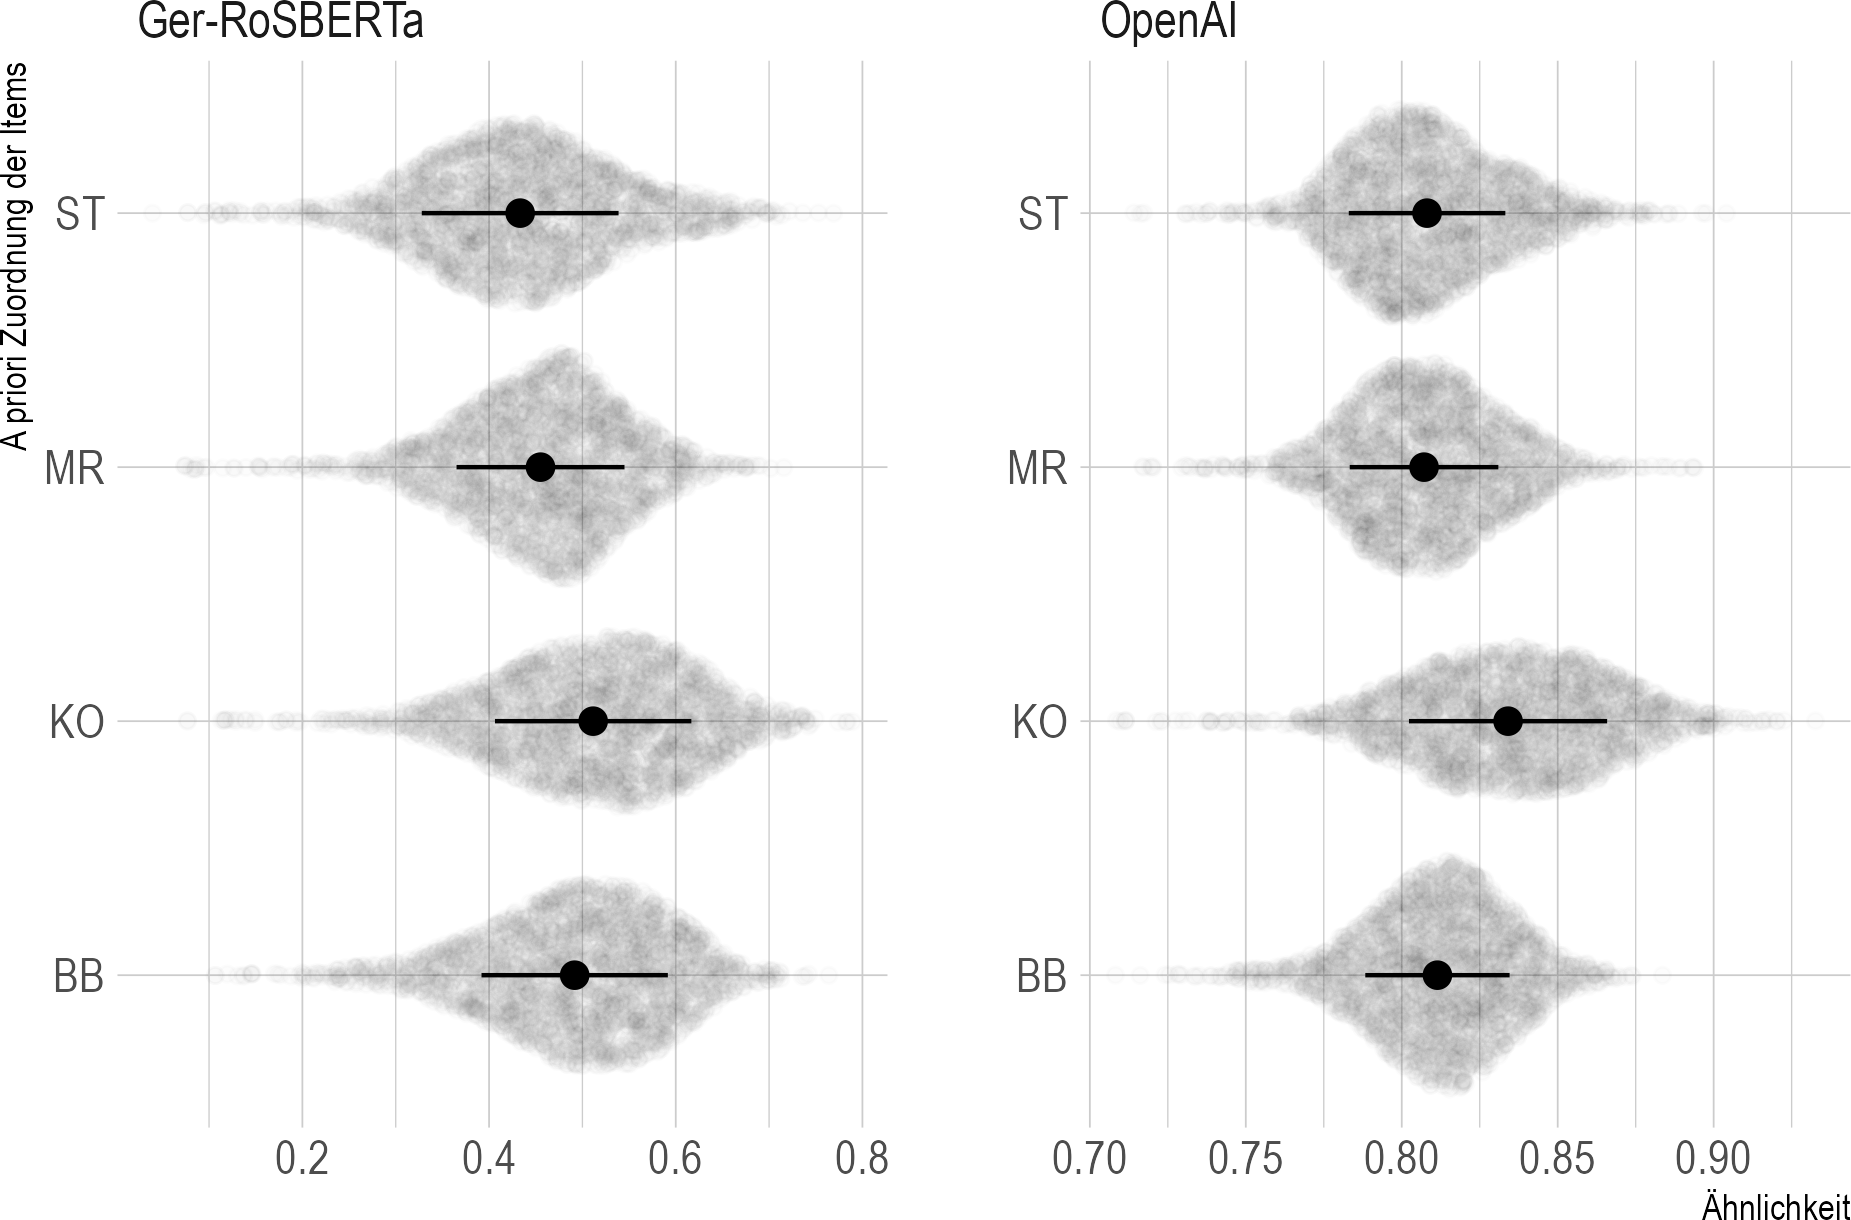
\includegraphics[keepaspectratio]{index_files/figure-pdf/fig-embeddings-1.png}}

}

\caption{\label{fig-embeddings}Ähnlichkeiten der offenen Antworten zu
allen Items, gegliedert nach deren a priori Dimensionen (ST =
strukturtheoretischer Ansatz, MR = Metareflektiver Ansatz, KO =
kompetenzorientierter Ansatz, BB = berufsbiographischer Ansatz).}

\end{figure}%

Um zu eruieren inwiefern diese offenen Antworten Ideen der vier unter
Kapitel~\ref{sec-professionalitat-von-lehrkraften} beschriebenen
bildungswissenschaftlichen Ansätze enthalten, wurde die Ähnlichkeit
aller Antworten zu allen Items des Instrumentes von Cramer et al (2023)
in zwei Transformermodellen bestimmt. Diese Ähnlichkeiten zeigten sich
als unimodal und sehr ähnlich in ihren Verteiungsformen über die beiden
gewählten Transformermodelle hinweg (siehe
Abbildung~\ref{fig-embeddings}).

\begin{table}

\caption{\label{tbl-embeddings}Deskriptive Verteilungsbeschreibung der
Ähnlichkeiten der offenen Antworten zu allen Items (ST =
strukturtheoretischer Ansatz, MR = Metareflektiver Ansatz, KO =
kompetenzorientierter Ansatz, BB = berufsbiographischer Ansatz).}

\centering{

\centering
\begin{tblr}[         %% tabularray outer open
]                     %% tabularray outer close
{                     %% tabularray inner open
colspec={Q[]Q[]Q[]Q[]Q[]Q[]Q[]Q[]Q[]},
}                     %% tabularray inner close
\toprule
Embedding & apriori_faktor & Min & Max & Med & MW & SD & Schiefe & Kurtosis \\ \midrule %% TinyTableHeader
Ger-RoSBERTa & BB & 0.107 & 0.76 & 0.5  & 0.49 & 0.1   & -0.565 & 3.4 \\
Ger-RoSBERTa & KO & 0.077 & 0.79 & 0.52 & 0.51 & 0.105 & -0.506 & 3.6 \\
Ger-RoSBERTa & MR & 0.074 & 0.72 & 0.46 & 0.46 & 0.09  & -0.61  & 4.2 \\
Ger-RoSBERTa & ST & 0.039 & 0.77 & 0.43 & 0.43 & 0.105 & -0.05  & 3.3 \\
OpenAI       & BB & 0.708 & 0.88 & 0.81 & 0.81 & 0.023 & -0.405 & 3.6 \\
OpenAI       & KO & 0.709 & 0.93 & 0.84 & 0.83 & 0.032 & -0.272 & 3.3 \\
OpenAI       & MR & 0.717 & 0.89 & 0.81 & 0.81 & 0.024 & 0.014  & 3.6 \\
OpenAI       & ST & 0.714 & 0.9  & 0.81 & 0.81 & 0.025 & 0.267  & 3.3 \\
\bottomrule
\end{tblr}

}

\end{table}%

Die unterschiedlichen Mittelwerte in Abbildung~\ref{fig-embeddings}
deuten auf eine Repräsentation der in den bildungswissenschaftlichen
Professionalitätsansätzen enthaltenen Ideen in den offenen Antworten
hin. Um diese auch inferenzstatistisch zu modellieren wurden
bayesianische Mehrebenen-Beta-Regressionsmodelle spezifiziert, in denen
die Ähnlichkeiten zwischen Itemwortlaut und Wortlaut der offenen Antwort
die abhängige Variable darstellten und dummykodierte Indikatorvariablen
der a priori Zuordnung der Variablen die unabhängige Variable. Um der
genesteten Struktur der Daten (mehrere Antworten pro Lehrkraft) Rechnung
zu tragen, wurden Random Intercepts im R-Paket brms (Bürkner 2017)
spezifiziert (siehe Listing~\ref{lst-reg01}), welches wiederum die
probabilistische Sprach Stan (Stan Development Team 2024) nutzt. Für
alle zu schätzenden Parameter wurden nicht-informative
Priorverteiltungen spezifiziert, wodurch die Punktschätzung vollständig
durch die Likelihood der Daten getrieben ist (Winter und Bürkner 2021)
(Lemoine 2019; Winter und Bürkner 2021). Die numerische Qualität der
vier unabhängigen Marcov-Chain-Monte-Carlo-Samplings wurde mithilfe von
Trace-Plots, \(\hat{R}\)-Werten sowie Bulk- und
Tail-Effective-Sample-Sizes bewertet.

\begin{codelisting}

\caption{\label{lst-reg01}}

\centering{

\begin{Shaded}
\begin{Highlighting}[]
\NormalTok{reg\_grosberta01 }\OtherTok{\textless{}{-}} 
  \FunctionTok{brm}\NormalTok{(}\FunctionTok{bf}\NormalTok{(similarity }\SpecialCharTok{\textasciitilde{}}\NormalTok{ apriori\_faktor }\SpecialCharTok{+}\NormalTok{ (}\DecValTok{1}\SpecialCharTok{|}\NormalTok{PID),}
\NormalTok{         phi }\SpecialCharTok{\textasciitilde{}}\NormalTok{ apriori\_faktor }\SpecialCharTok{+}\NormalTok{ (}\DecValTok{1}\SpecialCharTok{|}\NormalTok{PID)),}
      \AttributeTok{data =} 
\NormalTok{        data\_grosberta }\SpecialCharTok{\%\textgreater{}\%} 
        \FunctionTok{filter}\NormalTok{(spezifität }\SpecialCharTok{==} \StringTok{"Fachdidaktik"}\NormalTok{),}
      \AttributeTok{cores =} \DecValTok{4}\NormalTok{,}
      \AttributeTok{iter =} \DecValTok{6000}\NormalTok{,}
      \AttributeTok{family =} \FunctionTok{Beta}\NormalTok{(),}
      \AttributeTok{seed =} \DecValTok{1893}\NormalTok{)}
\FunctionTok{plot}\NormalTok{(reg\_grosberta01)}
\FunctionTok{pp\_check}\NormalTok{(reg\_grosberta01)}
\FunctionTok{summary}\NormalTok{(reg\_grosberta01)}

\NormalTok{reg\_openai01 }\OtherTok{\textless{}{-}} 
  \FunctionTok{brm}\NormalTok{(}\FunctionTok{bf}\NormalTok{(similarity }\SpecialCharTok{\textasciitilde{}}\NormalTok{ apriori\_faktor }\SpecialCharTok{+}\NormalTok{ (}\DecValTok{1}\SpecialCharTok{|}\NormalTok{PID),}
\NormalTok{         phi }\SpecialCharTok{\textasciitilde{}}\NormalTok{ apriori\_faktor }\SpecialCharTok{+}\NormalTok{ (}\DecValTok{1}\SpecialCharTok{|}\NormalTok{PID)),}
      \AttributeTok{data =} 
\NormalTok{        data\_openai }\SpecialCharTok{\%\textgreater{}\%} 
        \FunctionTok{filter}\NormalTok{(spezifität }\SpecialCharTok{==} \StringTok{"Fachdidaktik"}\NormalTok{),}
      \AttributeTok{cores =} \DecValTok{4}\NormalTok{,}
      \AttributeTok{iter =} \DecValTok{6000}\NormalTok{,}
      \AttributeTok{family =} \FunctionTok{Beta}\NormalTok{(),}
      \AttributeTok{seed =} \DecValTok{1893}\NormalTok{)}
\FunctionTok{plot}\NormalTok{(reg\_openai01)}
\FunctionTok{pp\_check}\NormalTok{(reg\_openai01)}
\FunctionTok{summary}\NormalTok{(reg\_openai01)}

\CommentTok{\# Da das MCMC Sampling zeitintensiv ist, werden die Objekte gespeichert}
\FunctionTok{save}\NormalTok{(reg\_grosberta01, reg\_openai01, }
     \AttributeTok{file =} \StringTok{"\_data/regs01.RData"}\NormalTok{)}
\end{Highlighting}
\end{Shaded}

}

\end{codelisting}%

Betrachtet man die bedingten Effekte dieser Modelle (siehe
Tabelle~\ref{tbl-conditional-effects-embeddings}), fällt auf, dass deren
Punktschätzung sehr gut mit den deskriptiven Ergebnissen korrespondiert
und die 95\%-Kredibilitätsintervalle sehr eng sind.

\begin{table}

\caption{\label{tbl-conditional-effects-embeddings}Bedingte Effekte der
Mehrebenen-Beta-Regressionsmodelle (ST = strukturtheoretischer Ansatz,
MR = Metareflektiver Ansatz, KO = kompetenzorientierter Ansatz, BB =
berufsbiographischer Ansatz).}

\centering{

\centering
\begin{tblr}[         %% tabularray outer open
]                     %% tabularray outer close
{                     %% tabularray inner open
colspec={Q[]Q[]Q[]},
cell{2}{1}={c=3}{},cell{7}{1}={c=3}{},
row{2,7}={}{halign=c,},
cell{3}{1}={}{preto={\hspace{1em}},},
cell{4}{1}={}{preto={\hspace{1em}},},
cell{5}{1}={}{preto={\hspace{1em}},},
cell{6}{1}={}{preto={\hspace{1em}},},
cell{8}{1}={}{preto={\hspace{1em}},},
cell{9}{1}={}{preto={\hspace{1em}},},
cell{10}{1}={}{preto={\hspace{1em}},},
cell{11}{1}={}{preto={\hspace{1em}},},
}                     %% tabularray inner close
\toprule
A priori Faktor & Ähnlichkeit & 95%-CI \\ \midrule %% TinyTableHeader
Ger-RoSBERTa Embeddings && \\
BB & 0.490 & [0.481; 0.499] \\
KO & 0.512 & [0.502; 0.521] \\
MR & 0.453 & [0.444; 0.462] \\
ST & 0.432 & [0.423; 0.441] \\
OpenAI Embeddings && \\
BB & 0.812 & [0.810; 0.814] \\
KO & 0.833 & [0.831; 0.835] \\
MR & 0.808 & [0.806; 0.810] \\
ST & 0.809 & [0.806; 0.811] \\
\bottomrule
\end{tblr}

}

\end{table}%

\subsubsection{Forschungsfrage 2}\label{sec-ergebnisseff2}

Da Forschungsfrage 2 sich für die Replikation der Ergebnisse von Cramer
et al. (2023) interessiert, wurde wie präregistriert die Passung dreier
konfirmatorischer Faktorenanalysen verglichen (siehe
Kapitel~\ref{sec-faktorenanalysen}).

Dabei zeigte sich auf den vorliegenden Daten (Stichprobe 1) passend zur
präregistrierten Hypothese der beste Fit für das a-Posteriori-Modell (χ²
= 120.300, \emph{df} = 62, RMSEA = 0.072, SRMR = 0.062, BIC = 6268.2,
AIC = 6175.5) im Vergleich zur eindimensionales Lösung (χ² = 222.900,
\emph{df} = 104, RMSEA = 0.080, SRMR = 0.073, BIC = 7478.0, AIC =
7376.2), welche wiederum dem a-priori-Modell (χ² = 185.400, \emph{df} =
98, RMSEA = 0.071, SRMR = 0.070, BIC = 7471.6, AIC = 7350.7) signifikant
unterlegen war (Δχ² = 37.503, Δ\emph{df} = 6.000, \emph{p} \textless{}
.001). Obwohl diese Ergebnisse der präregistrierten Hypothese
entsprechen, muss jedoch angemerkt werden, dass auch das empirisch
favorisierte Modell in einigen nicht-präregistrierten Fit-Indices (z.B.
Tucker Lewis Index {[}TLI{]}, Confirmatory Fit Index {[}CFI{]}) Werte
aufzeigen, die auf eine mangelnde Passung hinweisen (TLI = 0.850, CFI =
0.880) und zudem die Varianz-Kovarianz-Matrix der latenten Variablen des
a-priori-Modells nicht positiv definit war.

\subsubsection{Forschungsfrage 3}\label{forschungsfrage-3}

Zur Bearbeitung der Forschungsfrage 3 wurden zwei weitere Datensätze
hinzugezogen: Zum Vergleich der offen erfassten globalen und
fachdidaktik-spezifischen Professionalitätsüberzeugungen wurden
dieselben Regressionsmodelle wie in Kapitel~\ref{sec-word-embeddings}
spezifiziert, jedoch die Daten von Stichprobe 1 und 2 verwendent und um
Interaktionseffekte für die Domänenspezifität ergänzt (siehe
Listing~\ref{lst-reg02}).

\begin{codelisting}

\caption{\label{lst-reg02}}

\centering{

\begin{Shaded}
\begin{Highlighting}[]
\NormalTok{reg\_grosberta02 }\OtherTok{\textless{}{-}} 
  \FunctionTok{brm}\NormalTok{(}\FunctionTok{bf}\NormalTok{(similarity }\SpecialCharTok{\textasciitilde{}}\NormalTok{ apriori\_faktor}\SpecialCharTok{*}\NormalTok{spezifität }\SpecialCharTok{+}\NormalTok{ (}\DecValTok{1}\SpecialCharTok{|}\NormalTok{PID),}
\NormalTok{         phi }\SpecialCharTok{\textasciitilde{}}\NormalTok{ apriori\_faktor}\SpecialCharTok{*}\NormalTok{spezifität }\SpecialCharTok{+}\NormalTok{ (}\DecValTok{1}\SpecialCharTok{|}\NormalTok{PID)),}
      \AttributeTok{data =} 
\NormalTok{        data\_grosberta,}
      \AttributeTok{cores =} \DecValTok{4}\NormalTok{,}
      \AttributeTok{iter =} \DecValTok{6000}\NormalTok{,}
      \AttributeTok{family =} \FunctionTok{Beta}\NormalTok{(),}
      \AttributeTok{seed =} \DecValTok{1893}\NormalTok{)}
\FunctionTok{plot}\NormalTok{(reg\_grosberta02)}
\FunctionTok{pp\_check}\NormalTok{(reg\_grosberta02)}
\FunctionTok{summary}\NormalTok{(reg\_grosberta02)}

\NormalTok{reg\_openai02 }\OtherTok{\textless{}{-}} 
  \FunctionTok{brm}\NormalTok{(}\FunctionTok{bf}\NormalTok{(similarity }\SpecialCharTok{\textasciitilde{}}\NormalTok{ apriori\_faktor}\SpecialCharTok{*}\NormalTok{spezifität }\SpecialCharTok{+}\NormalTok{ (}\DecValTok{1}\SpecialCharTok{|}\NormalTok{PID),}
\NormalTok{         phi }\SpecialCharTok{\textasciitilde{}}\NormalTok{ apriori\_faktor}\SpecialCharTok{*}\NormalTok{spezifität }\SpecialCharTok{+}\NormalTok{ (}\DecValTok{1}\SpecialCharTok{|}\NormalTok{PID)),}
      \AttributeTok{data =} 
\NormalTok{        data\_openai,}
      \AttributeTok{cores =} \DecValTok{4}\NormalTok{,}
      \AttributeTok{family =} \FunctionTok{Beta}\NormalTok{(),}
      \AttributeTok{seed =} \DecValTok{1893}\NormalTok{)}
\FunctionTok{plot}\NormalTok{(reg\_openai02)}
\FunctionTok{pp\_check}\NormalTok{(reg\_openai02)}
\FunctionTok{summary}\NormalTok{(reg\_openai02)}

\CommentTok{\# Da das MCMC Sampling zeitintensiv ist, werden die Objekte gespeichert}
\FunctionTok{save}\NormalTok{(reg\_grosberta02, reg\_openai02, }
     \AttributeTok{file =} \StringTok{"\_data/regs02.RData"}\NormalTok{)}
\end{Highlighting}
\end{Shaded}

}

\end{codelisting}%

Die Interaktionseffekte sind in Abbildung~\ref{fig-cond-eff-reg-ff3}
dargestellt und zeigen im Wesentlichen eine sehr starke Überlappung der
Ähnlichkeiten der offenen Antworten zu den Items der
bildungswissenschaftlichen Professionalitätsansätze. Die Ähnlichkeiten
scheinen also relativ unabhängig davon zu sein, ob die Lehrkräfte dazu
aufgefordert wurden zu beschreiben was Professionalität im Lehrerinnen-
und Lehrerberuf ausmacht (globale Professionalitätsüberzeugung) oder was
Professionalität in der Fachdidaktik Deutsch (Sprache) ausmacht.
Gleichzeitig fällt auf, dass die Ähnlichkeiten (mit einer Ausnahme
\emph{d} = -0.07) der Antworten auf die Frage nach den globalen
Professionalitätsüberzeugungen etwas größer ausfallen (0.05 ≤ \emph{d} ≤
0.30). Dies ist plausibel, da die Items von Cramer et al. (2023), zu
denen die Ähnlichkeit der offenen Antworten bestimmt wurde, ebenfalls
globale Professionalitätsüberzeugungen erfassen.

\phantomsection\label{cell-fig-cond-eff-reg-ff3}
\begin{figure}[H]

\centering{

\pandocbounded{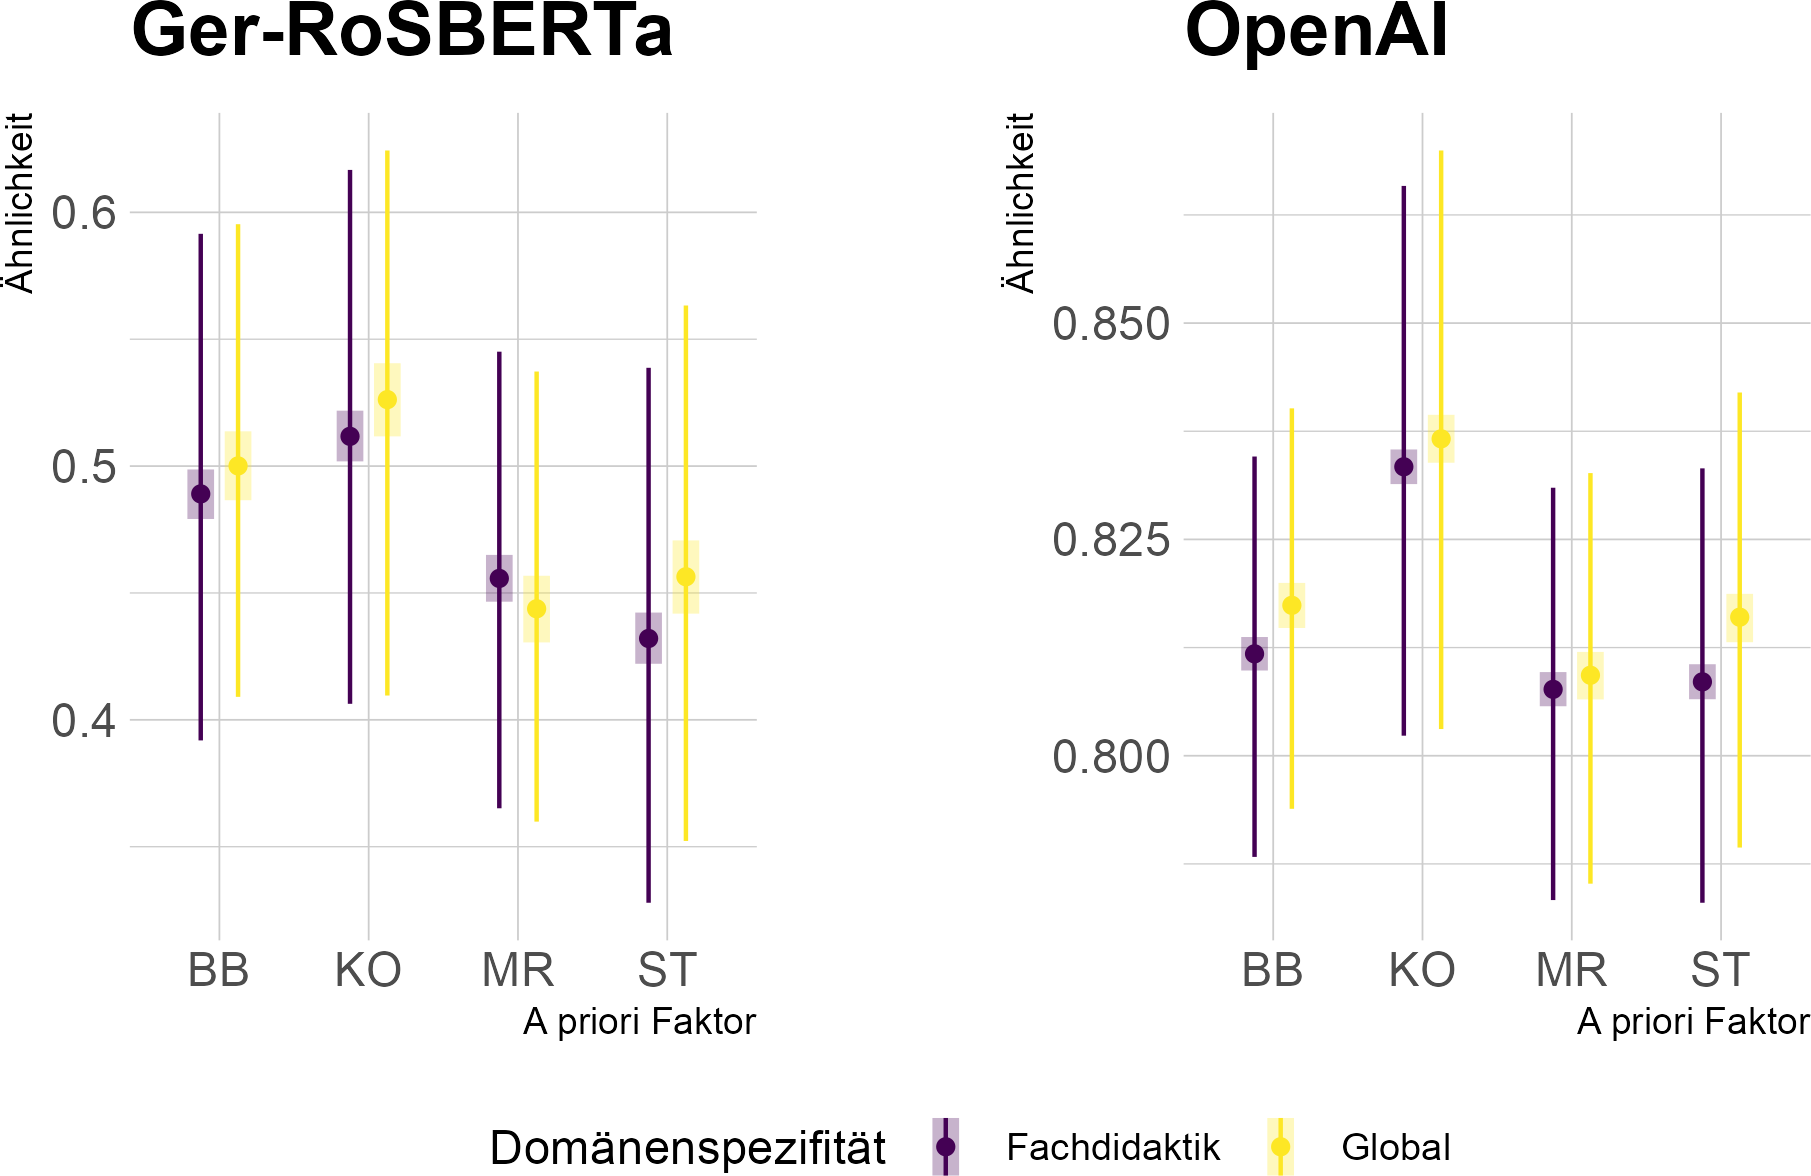
\includegraphics[keepaspectratio]{index_files/figure-pdf/fig-cond-eff-reg-ff3-1.png}}

}

\caption{\label{fig-cond-eff-reg-ff3}Bedingte Effekte der
Mehrebenen-Beta-Regressionsmodelle mit Interaktionseffekten für die
Domänenspezifität (Breites Intervall = 95\% Kredibilitätintervall,
schmales Intervall = MW ± 1SD, ST = strukturtheoretischer Ansatz, MR =
Metareflektiver Ansatz, KO = kompetenzorientierter Ansatz, BB =
berufsbiographischer Ansatz).}

\end{figure}%

Abschließend wurden konfirmatorische Zweigruppen-Faktorenanalysen
durchgeführt, um die Domänenspezifität auch auf Itemebene zu
untersuchen. Dabei wurde sowohl für die a priori als auch die a
posteriori Faktorenstruktur in einer Serie von Modellen sukzessive
Faktorenstruktur, Ladungen, Intercepts und Residualvarianzen der Items
als zwischen den Gruppen gleich restringiert (siehe
Kapitel~\ref{sec-faktorenanalysen}).

\begin{table}

\caption{\label{tbl-mgcfa-ff3}Fit Indices der Messinvarianzanalyse.}

\centering{

\centering
\begin{tblr}[         %% tabularray outer open
]                     %% tabularray outer close
{                     %% tabularray inner open
width={1\linewidth},
colspec={X[0.181818181818182]X[0.181818181818182]X[0.106060606060606]X[0.106060606060606]X[0.106060606060606]X[0.106060606060606]X[0.106060606060606]X[0.106060606060606]},
column{1,2,3,4,5,6,7,8}={}{font=\fontsize{0.8em}{1.1em}\selectfont,},
}                     %% tabularray inner close
\toprule
Struktur & Modell & χ² & df & CFI & SRMR & BIC & P(Δχ²) \\ \midrule %% TinyTableHeader
A priori     & Konfigural & 444.936 & 196 & 0.920 & 0.051 & 25981.70 & -     \\
A priori     & Metrisch   & 454.901 & 208 & 0.921 & 0.054 & 25915.21 & 0.619 \\
A priori     & Skalar     & 504.927 & 220 & 0.908 & 0.057 & 25888.77 & 0.000 \\
A priori     & Strikt     & 579.865 & 236 & 0.890 & 0.065 & 25861.76 & 0.000 \\
A posteriori & Konfigural & 251.698 & 124 & 0.944 & 0.043 & 21687.48 & -     \\
A posteriori & Metrisch   & 261.503 & 134 & 0.944 & 0.047 & 21633.51 & 0.458 \\
A posteriori & Skalar     & 299.290 & 144 & 0.932 & 0.051 & 21607.53 & 0.000 \\
A posteriori & Strikt     & 341.691 & 157 & 0.919 & 0.057 & 21567.04 & 0.000 \\
\bottomrule
\end{tblr}

}

\end{table}%

Die Ergebnisse dieser Messinvarianzanalyse in
Tabelle~\ref{tbl-mgcfa-ff3} können als Evidenz für die Annahme
metrischer Skaleninvarianz (gleiche Item-Intercepts) interpretiert
werden. Die Items wiesen also vorliegend die gleichen Ladungen auf,
unabhängig davon, ob nach einer professionellen Lehrperson oder einer
professionellen Lehrperson in der Deutsch-Fachdidaktik (Sprache) gefragt
wurde, jedoch unterschiedliche Intercepts und Residualvarianen.

\subsection{Diskussion (8K)}\label{diskussion-8k}

Die vorliegende Arbeit hat drei zentrale Ergebnisse: Erstens enthalten
offene Antworten von Lehrkräten auf die Frage, was »Professionalität« in
der Deutsch-Fachdidaktik (Sprache) bzw. im Allgemeinen ausmacht, die
Ideen bildungswissenschaftlicher Professionalitätsansätze
(strukturtheoretischer, metareflektiver, kompetenzorientierter und
berufsbiographischer Ansatz). Zweitens konnte im Instrument mit
geschlossenen Items zur Erfassung von Professionalitätsüberzeugungen von
Cramer at al. (2023) der Ausschluss einer eindimensionalen und einer a
priori Struktur (vier Faktoren für strukturtheoretischen,
metareflektiven, kompetenzorientierten und berufsbiographischen Ansatz)
repliziert werden. Die von Cramer at al. (2023) explorativ gefundene
Struktur zeigte die vergleichsweise besten Fit-Indizes, die jedoch unter
den klassischen Benchmarks für akzeptable oder gute Modellpassungen
liegen (McNeish und Wolf 2021). Drittens zeigen offen wie geschlossen
erfasste Professionalitätsüberzeugungen sowohl Aspekte von
Domänenspezifität als auch von Domänengeneralität: So sind etwa die
offenen Antworten auf den globalen Stimulus (\emph{Wir interessieren uns
nun dafür, was Ihrer Ansicht nach »Professionalität« einer Lehrperson
ausmacht}) im Durchschnitt etwas ähnlicher zu den geschlossenen Items
als die Antworten, die auf den fachdidaktik-spezifischen Stimulus
folgen.\\
Als zentrale Stärke der vorliegenden Studie kann sicher deren externe
Validität hervorgehoben werden: Forschungsfragen 1 \& 2 wurden mit einer
Stichprobe von aktiven Deutschlehrkräften bearbeitet, deren Größe a
priori mit einer Poweranalyse determiniert wurde. Für Forschungsfrage 3
wurde zudem eine repräsentative Stichprobe von Lehrkräften reanalysiert.
Dem stehen Schwächen der Studie - insbesondere die Konstruktvalidität
betreffend - entgehen. Und zwar sowohl bzgl. der geschlossenen als auch
der offenen Erfassung der Professionalitätsüberzeugungen: Die schwache
absolute Ausprägung der Fit-Indices der konfirmatischen Faktorenanalysen
lassen offenen, inwiefern die in Forschungsfrage 3 angestellten
Vergleiche globaler und domänenspezifischer
Professionalitätsüberzeugungen überhaupt sinnvoll sind, da unklar bleibt
inwiefern die von Cramer et al. (2023) postulierten Faktoren von
überhaupt existieren. Die Konstruktvalidität der für das Sentence
Embedding verwendeten Transformermodellen ist vielfach sehr positiv
beschrieben worden XXX. Nichts desto trotz wäre eine explizite
Überprüfung im vorliegenden Fall wünschenswert. So könnten geschulte
Kodiererinnen und Kodierer die offenen Antworten (siehe Open Data dieser
Studie) inhaltsanalytisch den bildungswissenschaftlichen
Professionalitätsansätzen zuordnen und dann prüfen, inwiefern diese mit
den Embeddings prädiziert werden können. Die vorliegende Evidenz für die
Ähnlichkeit offen erfasster Professionalitätsüberzeugungen zu
bildungswissenschaftlichen Ansätzen motiviert im Lichte der im
Theorieteil beschriebenen Filter-, Rahmungs- und
Handlungsleitungsfunktion von Überzeugungen (Fives und Buehl 2012) auch
anwendungsbezogenere Folgeforschung: So stellt sich etwa die Frage ob
Professionalitätsüberzeugungen die aus bildungswissenschaftlicher Sicht
eher als überholt zu bewerten sind (z.B. eine bestimmte ``Lehrerinnen-
und Lehrerpersönlichkeit'' als zentrales Merkmal von Professionalität)
im Sinne eines Bestätigungsfehlers (``Confirmation Bias'', Bohrer,
Schmidt, und Merk 2025; Nickerson 1998; Masnick und Zimmerman 2009) zur
abwertenden Evaluation von empirischen Ergebnissen der Studien führen,
die einen anderen Professionalitätsansatz verfolgen. Auch die Wahl von
Veranstaltungen in der ersten Phase der Lehrerbildung oder
Entscheidungen für oder gegen bestimmte Fortbildungen in der dritten
Phase könnte durch die Handlungsleitungsfunktion von
Professionalitätsüberzeugungen beeinflusst werden. Ließe sich Evidenz
für diese Funktion der Professionalisierungsüberzeugungen finden, wäre
ein konsequenter nächster Schritt zu untersuchen inwiefern
Awarenessinterventionen die darauf aufmerksam machen, dass Individuen
solche Überzeugungen besitzen und diese ihre Entscheidungen beeinflussen
oder andere Deboiasingn Strategien wie ``Consider the Opposite''
(Brussel u.~a. 2020) zu einem weniger durch die Überzeugungen verzerrten
und reflektierteren Handeln führen.

\section{Anhang}\label{anhang}

\subsubsection{Wortlaut der Items}\label{sec-wortlaut-der-items}

\paragraph{Offene Items}\label{offene-items}

\begin{itemize}
\tightlist
\item
  Wir interessieren uns nun dafür, was Ihrer Ansicht nach
  »Professionalität« in der Deutsch-Fachdidaktik (Sprache) ausmacht.
  Bitte antworten Sie in ganzen Sätzen um Missverständnisse zu vermeiden
  und formulieren Sie möglichst drei Aspekte. Eine »professionelle«
  Lehrperson in der Deutsch-Fachdidaktik (Sprache) \ldots{}
\item
  Wir interessieren uns nun dafür, was Ihrer Ansicht nach
  »Professionalität« einer Lehrperson ausmacht. Bitte antworten Sie in
  ganzen Sätzen um Missverständnisse zu vermeiden und formulieren Sie
  möglichst drei Aspekte. Eine »professionelle« Lehrperson \ldots{}
\end{itemize}

\paragraph{Geschlossene Items}\label{sec-geschlossene-items}

siehe XXX

\phantomsection\label{refs}
\begin{CSLReferences}{1}{0}
\bibitem[\citeproctext]{ref-bauer2000}
Bauer, K.-O. 2000. {„Pädagoge - Profession und Nebenbeschäftigung?``}
In, herausgegeben von O Jaumann-Graumann und W Köhnlein, 25--44.

\bibitem[\citeproctext]{ref-baumert2006}
Baumert, Jürgen, und Mareike Kunter. 2006. {„Stichwort: Professionelle
Kompetenz von Lehrkräften``}. \emph{Zeitschrift für
Erziehungswissenschaft} 9 (4): 469--520.
\url{https://doi.org/10.1007/s11618-006-0165-2}.

\bibitem[\citeproctext]{ref-Bell2011}
Bell, Sherrilee. 2011. {„Professionalism through the eyes of female
elementary teachers in Ontario``}. Phdthesis, Kingston.
\href{http://\%20hdl.handle.net/1974/6468}{http://
hdl.handle.net/1974/6468}.

\bibitem[\citeproctext]{ref-bittermann2024}
Bittermann, André, und Andreas Fischer. 2024. {„Natural Language
Processing in Psychology``}. \emph{Zeitschrift für Psychologie} 232 (3):
143--46. \url{https://doi.org/10.1027/2151-2604/a000568}.

\bibitem[\citeproctext]{ref-bluxf6meke2008}
Blömeke, Sigrid, Christiane Müller, Anja Felbrich, und Gabriele Kaiser.
2008. {„Epistemologische Überzeugungen zur Mathematik``}. In,
herausgegeben von Sigrid Blömeke, Gabriele Kaiser, und Rainer Lehmann,
219--46. Münster: Waxmann.

\bibitem[\citeproctext]{ref-bohrer2025}
Bohrer, Kristina, Kirstin Schmidt, und S. Merk. 2025. {„{Zwei Studien,
ein Ergebnis: Lehramtsstudierende unterliegen im Umgang mit Evidenz dem
Ankereffekt}``}. \emph{Zeitschrift für Erziehungswissenschaft}.

\bibitem[\citeproctext]{ref-bromme1992}
Bromme, Rainer. 1992. \emph{Der Lehrer als Experte: Zur Psychologie des
professionellen Wissens}. Bern u.a.: H. Huber.

\bibitem[\citeproctext]{ref-vanbrussel2020}
Brussel, Suzan van, Miranda Timmermans, Peter Verkoeijen, und Fred Paas.
2020. {„{`}Consider the Opposite{'} {\textendash} Effects of Elaborative
Feedback and Correct Answer Feedback on Reducing Confirmation Bias
{\textendash} A Pre-Registered Study``}. \emph{Contemporary Educational
Psychology} 60 (Januar): 101844.
\url{https://doi.org/10.1016/j.cedpsych.2020.101844}.

\bibitem[\citeproctext]{ref-buxfcrkner2017}
Bürkner, Paul-Christian. 2017. {„Brms: An R Package for Bayesian
Multilevel Models Using Stan``}. \emph{Journal of Statistical Software}
80 (1). \url{https://doi.org/10.18637/jss.v080.i01}.

\bibitem[\citeproctext]{ref-cramer2019}
Cramer, C., M. Harant, S. Merk, M. Drahmann, und M. Emmerich. 2019.
{„Meta-Reflexivität und Professionalität im Lehrerinnen- und
Lehrerberuf``}. \emph{Zeitschrift für Pädagogik} 65 (3): 401--23.

\bibitem[\citeproctext]{ref-cramer2023a}
Cramer, Colin, Chris Brown, und David Aldridge. 2023. {„Meta-Reflexivity
and Teacher Professionalism: Facilitating Multiparadigmatic Teacher
Education to Achieve a Future-Proof Profession``}. \emph{Journal of
Teacher Education}, April, 00224871231162295.
\url{https://doi.org/10.1177/00224871231162295}.

\bibitem[\citeproctext]{ref-cramer2023}
Cramer, Colin, Jana Groß Ophoff, und Felix Schreiber. 2023.
{„Professionalität im Lehrerinnen- und Lehrerberuf``}.

\bibitem[\citeproctext]{ref-dubberke2008}
Dubberke, Thamar, Mareike Kunter, Nele McElvany, Martin Brunner, und
Jürgen Baumert. 2008. {„Lerntheoretische Überzeugungen von
Mathematiklehrkräften. Einflüsse auf die Unterrichtsgestaltung und den
Lernerfolg von Schülerinnen und Schülern``}. \emph{Zeitschrift für
Pädagogische Psychologie} 22 (3-4): 193--206.
\url{https://doi.org/10.1024/1010-0652.22.34.193}.

\bibitem[\citeproctext]{ref-fives2019}
Fives, Helenrose, Nicole Barnes, Candice Chiavola, Kit SaizdeLaMora,
Erika Oliveros, und Sirine Mabrouk-Hattab. 2019. {„Reviews of
Teachers{'} Beliefs``}. In. Oxford University Press.
\url{https://doi.org/10.1093/acrefore/9780190264093.013.781}.

\bibitem[\citeproctext]{ref-fives2008}
Fives, Helenrose, und Michelle M. Buehl. 2008. {„What do teachers
believe? Developing a framework for examining beliefs about teachers'
knowledge and ability``}. \emph{Contemporary Educational Psychology} 33
(2): 134--76. \url{https://doi.org/10.1016/j.cedpsych.2008.01.001}.

\bibitem[\citeproctext]{ref-fives2012}
---------. 2012. {„Spring Cleaning for the {``}Messy{''} Construct of
Teachers{'} Beliefs: What Are They? Which Have Been Examined? What Can
They Tell Us?``} In, herausgegeben von Karen R. Harris, Steve Graham,
Tim Urdan, Sandra Graham, James M. Royer, und Moshe Zeidner, 471--99.
Washington: American Psychological Association.
\url{https://doi.org/10.1037/13274-019}.

\bibitem[\citeproctext]{ref-gebauer2013}
Gebauer, Miriam M, Nele McElvany, und Stephanie Klukas. 2013.
{„Einstellungen von Lehramtsanwärterinnen und Lehramtsanwärtern zum
Umgang mit heterogenen Schülergruppen in Schule und Unterricht``}.
\emph{Jahrbuch der Schulentwicklung}, Nr. 17: 191--216.

\bibitem[\citeproctext]{ref-gold2024}
Gold, Bernadette, Eva Thomm, und Johannes Bauer. 2024. {„Using the
Theory of Planned Behaviour to Predict Pre‐service Teachers' Preferences
for Scientific Sources``}. \emph{British Journal of Educational
Psychology} 94 (1): 216--30. \url{https://doi.org/10.1111/bjep.12643}.

\bibitem[\citeproctext]{ref-greene2024}
Greene, Ryan, Ted Sanders, Lilian Weng, und Arvind Neelakatan. 2024.
{„New and Improved Embedding Model Ryan Greene, Ted Sanders, Lilian
Weng, Arvind Neelakantan``}.
\url{https://openai.com/index/new-and-improved-embedding-model/}.

\bibitem[\citeproctext]{ref-helsper2014}
Helsper, Werner. 2014. {„Lehrerprofessionalität - der
strukturtheoretische Professionsansatz zum Lehrerberuf``}. In,
herausgegeben von Ewald Terhart, Hedda Bennewitz, und Martin Rothland,
216240. Münster: Waxmann.

\bibitem[\citeproctext]{ref-hofer2012}
Hofer, B. K., und Lisa D Bendixen. 2012. {„Personal epistemology:
Theory, research, and future directions``}. In, herausgegeben von Karen
R Harris, Steve Graham, Tim Urdan, Christine B McCormick, Gale M
Sinatra, und John Sweller, 227--56. Washington: American Psychological
Association. \url{https://doi.org/10.1037/13273-009}.

\bibitem[\citeproctext]{ref-hohenstein2014}
Hohenstein, Friederike, Friederike Zimmermann, Thilo Kleickmann, Olaf
Köller, und Jens Möller. 2014. {„Sind die bildungswissenschaftlichen
Standards für die Lehramtsausbildung in den Curricula der Hochschulen
angekommen?``} \emph{Zeitschrift für Erziehungswissenschaft} 17 (3):
497--507. \url{https://doi.org/10.1007/s11618-014-0563-9}.

\bibitem[\citeproctext]{ref-kjell2023}
Kjell, Oscar, Salvatore Giorgi, und H. Andrew Schwartz. 2023. {„The
Text-Package: An R-Package for Analyzing and Visualizing Human Language
Using Natural Language Processing and Transformers.``}
\emph{Psychological Methods} 28 (6): 1478--98.
\url{https://doi.org/10.1037/met0000542}.

\bibitem[\citeproctext]{ref-konig2020}
König, Johannes. 2020. {„Kompetenzorientierter Ansatz in der
Lehrerinnen- und Lehrerbildung``}. In, herausgegeben von Colin Cramer,
Johannes König, Martin Rothland, und Sigrid Blömeke. Verlag Julius
Klinkhardt. \url{https://doi.org/10.35468/hblb2020-019}.

\bibitem[\citeproctext]{ref-krauss2004}
Krauss, Stefan, Mareike Kunter, Martin Brunner, Jürgen Baumert, W Blum,
Michael Neubrand, Alexander Jordan, und K Löwen. 2004. {„COACTIV.
Professionswissen von Lehrkräften, kognitiv aktivierender
Mathematikunterricht und die Entwicklung von mathematischer
Kompetenz``}. In, herausgegeben von M Doll und M Prenzel, 31--53.
Münster: Waxmann.
\url{https://books.google.de/books?id=EojWGyRAzAkC&lpg=PP1&hl=de&pg=PA21&redir_esc=y\#v=onepage&q&f=false}.

\bibitem[\citeproctext]{ref-lakens2022}
Lakens, Daniël. 2022. {„Sample Size Justification``}. \emph{Collabra:
Psychology} 8 (1): 33267. \url{https://doi.org/10.1525/collabra.33267}.

\bibitem[\citeproctext]{ref-lemoine2019}
Lemoine, Nathan P. 2019. {„Moving Beyond Noninformative Priors: Why and
How to Choose Weakly Informative Priors in Bayesian Analyses``}.
\emph{Oikos} 128 (7): 912--28. \url{https://doi.org/10.1111/oik.05985}.

\bibitem[\citeproctext]{ref-luong2021}
Luong, Raymond, und Jessica Kay Flake. 2021. {„Measurement Invariance
Testing Using Confirmatory Factor Analysis and Alignment Optimization: A
Tutorial for Transparent Analysis Planning and Reporting``}, September.
\url{https://doi.org/10.31234/osf.io/qr32u}.

\bibitem[\citeproctext]{ref-masnick2009}
Masnick, Amy M., und Corinne Zimmerman. 2009. {„Evaluating Scientific
Research in the Context of Prior Belief: {Hindsight} Bias or
Confirmation Bias?``} \emph{Journal of Psychology of Science and
Technology} 2 (1): 29--36.
\url{https://doi.org/10.1891/1939-7054.2.1.29}.

\bibitem[\citeproctext]{ref-mcneish2021}
McNeish, Daniel, und Melissa G. Wolf. 2021. {„Dynamic Fit Index Cutoffs
for Confirmatory Factor Analysis Models``}. \emph{Psychological
Methods}, Oktober. \url{https://doi.org/10.1037/met0000425}.

\bibitem[\citeproctext]{ref-merk2020}
Merk, S. 2020. {„Überzeugungen``}. In, herausgegeben von Colin Cramer,
Johannes König, Martin Rothland, und Sigrid Blömeke. Verlag Julius
Klinkhardt. \url{https://doi.org/10.35468/hblb2020-102}.

\bibitem[\citeproctext]{ref-merk2017}
Merk, S., Augustin Kelava, Jürgen Schneider, Marcus Syring, und Thorsten
Bohl. 2017. {„Teacher students{'} epistemic beliefs about general
pedagogical knowledge: Topic-, source- and context specificity``}.
\emph{Journal for Educational Research Online} 9 (1): 169--89.

\bibitem[\citeproctext]{ref-merk2023}
Merk, S., und Kirstin Schmidt. 2023. {„Grundlegende Fragen an eine
quantitativ-empirische Erfassung von Meta-Reflexivität``}. In,
herausgegeben von Colin Cramer, 143--54. Waxmann Verlag GmbH.
\url{https://doi.org/10.31244/9783830998068}.

\bibitem[\citeproctext]{ref-muis2006}
Muis, Krista R, Lisa D. Bendixen, und Florian C. Haerle. 2006.
{„Domain-Generality and Domain-Specificity in Personal Epistemology
Research: Philosophical and Empirical Reflections in the Development of
a Theoretical Framework``}. \emph{Educational Psychology Review} 18 (1):
3--54. \url{https://doi.org/10.1007/s10648-006-9003-6}.

\bibitem[\citeproctext]{ref-nickerson1998}
Nickerson, Raymond S. 1998. {„Confirmation Bias: {A} Ubiquitous
Phenomenon in Many Guises``}. \emph{Review of General Psychology} 2 (2):
175--220. \url{https://doi.org/10.1037/1089-2680.2.2.175}.

\bibitem[\citeproctext]{ref-oevermann1996}
Oevermann, U. 1996. {„Theoretische Skizze einer revidierten Theorie
professionalisierten Handelns``}. In, herausgegeben von A Combe und
Werner Helsper, 70--82. Frankfurt am Main: Suhrkamp.

\bibitem[\citeproctext]{ref-pajares1992}
Pajares, M. Frank. 1992. {„Teachers{'} Beliefs and Educational Research:
Cleaning up a Messy Construct``}. \emph{Review of Educational Research}
62 (3): 307--32. \url{https://doi.org/10.3102/00346543062003307}.

\bibitem[\citeproctext]{ref-reimers2019}
Reimers, Nils, und Iryna Gurevych. o.~J. {„Sentence-BERT: Sentence
Embeddings using Siamese BERT-Networks``}.
\url{https://doi.org/10.48550/ARXIV.1908.10084}.

\bibitem[\citeproctext]{ref-reusser2014}
Reusser, Kurt, und Christine Pauli. 2014. {„Berufsbezogene Überzeugungen
von Lehrerinnen und Lehrern``}. In, herausgegeben von Ewald Terhart,
Martin Rothland, und Hedda Bennewitz, 2. Aufl., 642--61. Münster:
Waxmann.

\bibitem[\citeproctext]{ref-robitzsch2022}
Robitzsch, Alexander, und Oliver Lüdtke. 2022. {„Why Measurement
Invariance is Not Necessary for Valid Group Comparisons``}.
\url{https://doi.org/10.31234/osf.io/cjyqp}.

\bibitem[\citeproctext]{ref-shulman1986}
Shulman, Lee S. 1986. {„Those who understand: Knowledge growth in
teaching``}. \emph{Educational Researcher} 15 (2): 4--14.
\url{https://doi.org/10.3102/0013189X015002004}.

\bibitem[\citeproctext]{ref-skott2015}
Skott, Jeppe. 2015. {„The Promises, Problems, and Prospects of Research
on Teachers{'} Beliefs``}. In, herausgegeben von H. Fives und Michele
Gregoire Gill, 1:13--30. New York: Routledge.

\bibitem[\citeproctext]{ref-standevelopmentteam2024}
Stan Development Team. 2024. \emph{Stan Modeling Language Users Guide
and Reference Manual}. \url{https://mc-stan.org}.

\bibitem[\citeproctext]{ref-terhart1992}
Terhart, E. 1992. {„Lehrerberuf und Professionalität``}. In,
herausgegeben von B Dewe, W Ferchhoff, und E O Radtke, 103--31. Opladen:
Leske u. Budrich.

\bibitem[\citeproctext]{ref-terhart1995c}
Terhart, Ewald. 1995. {„Lehrerprofessionalität``}. In, herausgegeben von
Hans-G. Rolff, 225266. Weinheim: Deutscher Studien Verlag.

\bibitem[\citeproctext]{ref-terhart2001}
---------. 2001. \emph{Lehrerberuf und Lehrerbildung. Forschungsbefunde,
Problemanalysen, Reformkonzepte}. Weinheim u.a.: Beltz.

\bibitem[\citeproctext]{ref-tschannen-moran2015}
Tschannen-Moran, Megan, Serena J. Salloum, und Roger D. Goddard. 2015.
{„Context Matters: The Influence of Collective Beliefs and Shared
Norms``}. In, herausgegeben von H. Fives und Michele Gregoire Gill, 1.
Aufl., 301--16. New York, NY: Routledge.
\url{http://gen.lib.rus.ec/book/index.php?md5=a59e2e3d2972bbc4b2610ee90c58fa33}.

\bibitem[\citeproctext]{ref-turner2009}
Turner, Julianne C., Andrea Christensen, und Debra K. Meyer. 2009.
{„Teachers' Beliefs about Student Learning and Motivation``}. In
\emph{International {Handbook} of {Research} on {Teachers} and
{Teaching}}, herausgegeben von Lawrence J. Saha und A. Gary Dworkin,
361--71. Boston, MA: Springer US.
\url{https://doi.org/10.1007/978-0-387-73317-3_23}.

\bibitem[\citeproctext]{ref-walker2019}
Walker, Matt, Julie Nelson, und Sally Bradshaw. 2019. {„Teachers'
Engagement with Research: What Do We Know? {A} Research Briefing.``}
Education Endowment Foundation.
\url{https://files.eric.ed.gov/fulltext/ED620325.pdf}.

\bibitem[\citeproctext]{ref-winter2021}
Winter, Bodo, und Paul-Christian Bürkner. 2021. {„Poisson Regression for
Linguists: A Tutorial Introduction to Modelling Count Data with Brms``}.
\emph{Language and Linguistics Compass} 15 (11).
\url{https://doi.org/10.1111/lnc3.12439}.

\bibitem[\citeproctext]{ref-zembylas2015}
Zembylas, Michalinos, und Sharon M. Chubbuck. 2015. {„The {Intersection}
of {Identity}, {Beliefs}, and {Politics} in {Conceptualizing} {‚{Teacher
Identity}`}``}. In \emph{International Handbook of Research on Teachers'
Beliefs}, herausgegeben von H. Fives und Michele Gregoire Gill, 1.
Aufl., 173--90. Routledge.
\url{http://gen.lib.rus.ec/book/index.php?md5=a59e2e3d2972bbc4b2610ee90c58fa33}.

\end{CSLReferences}




\end{document}
